%%%%%%%%%%%%%%%%%%%%%%%%%%%%%%%%%%%%%%%%%%%%%%%%%%%%%%%%%%%%%%%%%%%%%%%%%%%%%
\chapter{Practical Part}\label{chap:practicalPart}
%%%%%%%%%%%%%%%%%%%%%%%%%%%%%%%%%%%%%%%%%%%%%%%%%%%%%%%%%%%%%%%%%%%%%%%%%%%%%
\chapterstart

Your text here \ldots
\section{Use Case}
This use case is entirely fictional but allows the reader to get a better understanding of the circumstances a that led to the design of a federated authentication solution. The scenario features a medium to large company with up to 1000 employees. The mission of the company is to provide a network and analyzing toolset which allows the customer of the product suite to improve security within his network and keep an overview of potential security risks. Previously the customers received monthly reports about their current state of the network. Each of the products and tools resulted in a separate report which was sent via E-Mail. To modernize the approach, the reports should be replaced by a modern single-page application that could be accessed by customers and by employees for administrative reasons. In this example, we call the solution 'Security Assessment Portal.' The Security Assessment Portal should give the customers an overview of current products and the performance of the network an example of the suit could be E-Mail-filtering.  

The company already has a particular set of internal applications that are used by the employees within the company network. The company internally uses active directory for authorization on local machines. All applications until now are accessible within the companies network and use windows authentication. The application should be accessible by employees as well as customers whereas customers should not receive access to the company network. The data of the customers are sensible and therefore worth protecting. Because of the highly sensible data, certain customer do not need which to authenticate with an external provider. The application should be hosted within the company a solution for customers to access the application from outside is needed.


\section{Risk Assessment}



\section{Solution}
The \cite{Sakimura:2014:OpenIDConnect} explains that modern applications have different requirements than their predecessor due to new distributed architectures that allow enterprises to be more flexible. Cloud or Microservice architectures require different interactions between applications as the \ref{fig:architecture-identityserver} below show the most common interactions for modern applications.

\begin{figure}[h]
	\centering
	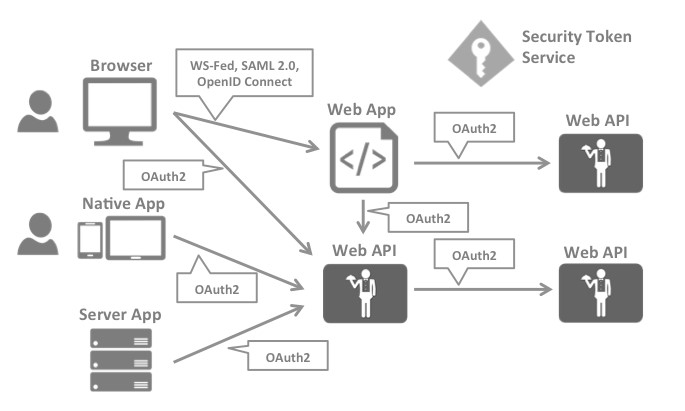
\includegraphics[width=0.8\linewidth]{images/architecture-identityserver}
	\caption[Architecture IdentityServer4]{}
	\caption{}
	\label{fig:architecture-identityserver}
\end{figure}



For example, a browser might call a Web App, and a Web App calls a Web API or perhaps a Native App calls a Web API, which is calling another Web API. Each application has to implement security functions to maintain a secure flow throughout these interactions, Implementing this security features for each involved application leads to a lot of duplicated code and inconsistencies. A different approach to implement security throughout these flows is using a token service. A token service brings the benefit of being able to encapsulate these security functions. Security functions can be updated and hosted at a single point which prevents duplicated functions across applications and security flaws [cf. (\cite{Sakimura:2014:OpenIDConnect})].

Identity Server4 is an ASP.NET framework that uses the specifics of OpenID Connect and OAuth 2.0 to enable Authentication and Authorization related features. Features include Authentication as a Service, which provides a centralized login logic for all applications, Single sign-on, Access Control for APIs and Federation Gateway. The Identity Server 4 will be used as a Token Server in the practical part [cf. (\cite{Brock:2018:ID4})]

The project illustrating the use of Identity Server and the benefits of OpenID Connect an OAuth is a Visual Studio Project mostly written in C\# and Typescript. The project example for Identity Server includes four different projects:

\begin{itemize}
	\item Identity Server - The Identity Server is a .NetCore Project with basic Implementation of an Identity Server which serves as a Token Server. 
	\item ProjectApiNetCore - This application is a .NetCore2.0 API Application with basic API that returns the users Claims if he is authenticated.
	\item Angular Client - The Angular Client is a .NetCore MVC Angular Project used as a Client that can be accessed by an End-User who can authenticate with the Identity Server and requests protected resources of the API ProjectApiNetCore.This project uses the Implicit Code Flow. 
	\item MVC Client - The MVC Client is a .Net Core MVC Project used as a Client that can be accessed by an End-User and can authenticate with the Identity Server and requests protected resources of the API ProjectApiNetCore. This project uses the Hybrid Code Flow. 
\end{itemize}



\paragraph{Identity Server}

This project is using the IdentityServer4 library by Brock Allen and Dominick Baier. The Project works as an Token Server which means that the Identity Server Project is responsible for authentication the user, managing the identities and provide and approve tokens. Furthermore the Identity Server implements different Authentication Flows. For the baisc Setup the Identity Server has to be added to the StartUp class and to ensure a secure communication a certificate has is created to sign request. For the basic setup Idenity Server provides us with DeveloperSigningCredentials which provides an dummy certificate. In this example application a real certificate is included. 

\begin{figure}[h]
	\centering
	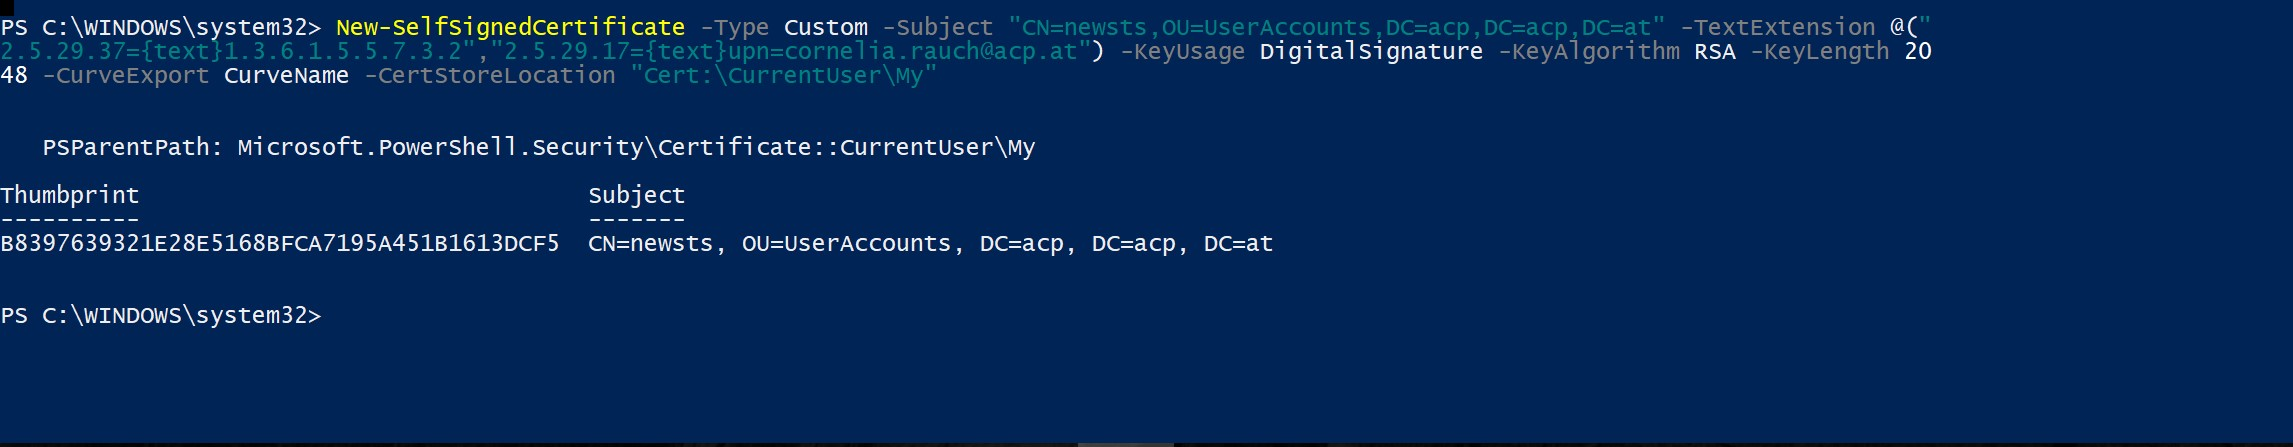
\includegraphics[width=0.8\linewidth]{images/self-signed-certicate}
	\caption{Self signed Certicate with Powershell}
	\label{fig:self-signed-certicate}
\end{figure}

The certificate used in this application was created with Powershell like shown in \ref{fig:self-signed-certicate}. The algorithm used in this certificate is RSA. Depending on the algorith that is used in the certificate a corresponding hashing algorith has to be used for the Client Secret.


The API Resources include the available APIs that can be called and included in the scope of a request. The Identity Resources are Resources that can be included in the returning id\_token. The Clients are the available Clients that can be configured and are able to use the Identity Server. Those Client Configurations indicate which Authorization Flow is used and how to retrive id\_token, access\_token and a possible refreh\_token. For simplifying reasons Identity Server provides an in Memory User Storage which can be used for Testing reasons. Other ways to define Users are via .NET Core Identity or IdentityServer4 EntityFramework. For the purpose of this implementation this Test Users where included in the Identity Server application:
\begin{enumerate}
	\item User1

	\begin{itemize}
	\item	Username: bob
	\item  Password: bob
\end{itemize} 

	\item User2

\begin{itemize}
	\item	Username: alice
	\item  Password: alice
\end{itemize} 

\end{enumerate}

\chapterend
